\chapter{PHÂN TÍCH HƯỚNG ĐỐI TƯỢNG}

Chương này chuyển các yêu cầu và trường hợp sử dụng đã xác định ở Chương 2 thành mô hình phân tích hướng đối tượng. Trọng tâm của chương là nhận diện lớp phân tích, phân loại theo Boundary--Control--Entity và đối chiếu các lớp này với từng trường hợp sử dụng chính của hệ thống.

\section{Cơ sở phân tích hướng đối tượng}

Phân tích hướng đối tượng ở giai đoạn này tập trung vào bài toán nghiệp vụ, chưa đi vào lớp triển khai, repository, bảng dữ liệu hay framework cụ thể. Các lớp phân tích được rút ra từ actor, trường hợp sử dụng, luồng hoạt động, yêu cầu chức năng, yêu cầu phi chức năng và các khái niệm nghiệp vụ xuất hiện trong miền bài toán.

Đề tài sử dụng cách phân loại Boundary--Control--Entity để tách trách nhiệm của lớp phân tích:

\begin{description}
    \item[Lớp biên] Đại diện cho điểm tương tác giữa actor hoặc hệ thống ngoài với Asymptotic. Lớp biên nhận yêu cầu, trả kết quả và che giấu chi tiết giao tiếp với bên ngoài.
    \item[Lớp điều khiển] Điều phối một trường hợp sử dụng hoặc một nhóm trách nhiệm nghiệp vụ. Lớp điều khiển không chỉ chuyển tiếp dữ liệu mà còn quyết định thứ tự kiểm tra định danh, chính sách, ngân sách, định tuyến và ghi nhận kết quả.
    \item[Lớp thực thể] Biểu diễn các khái niệm nghiệp vụ có trạng thái và vòng đời riêng như tổ chức, Agent, ví, chính sách ngân sách, giao dịch, bút toán, provider và trace.
\end{description}

Việc tách ba nhóm lớp giúp tránh đưa chi tiết thiết kế vào Chương 3. Ví dụ, việc Gateway kiểm soát request AI cần được phân tích bằng các lớp như \textit{AIRequestControl}, \textit{BudgetControl}, \textit{Agent}, \textit{Wallet} và \textit{ExecutionTrace}; còn handler, repository, adapter hoặc transaction manager sẽ được trình bày ở Chương 4.

\section{Nhận diện lớp phân tích}

Các lớp phân tích được nhận diện từ ba nguồn chính. Thứ nhất là các actor và hệ thống ngoài: AI Agent, quản trị viên tổ chức, lập trình viên, quản trị viên hệ thống, AI Provider và Payment Provider. Thứ hai là các use case trọng tâm như thực hiện yêu cầu AI qua Gateway, đăng ký AI Agent, cấp API key, nạp tiền, phân bổ ngân sách và theo dõi usage/cost/trace. Thứ ba là các thực thể nghiệp vụ cần lưu trạng thái để bảo đảm kiểm soát tài chính và truy vết.

\begin{figure}[H]
    \centering
    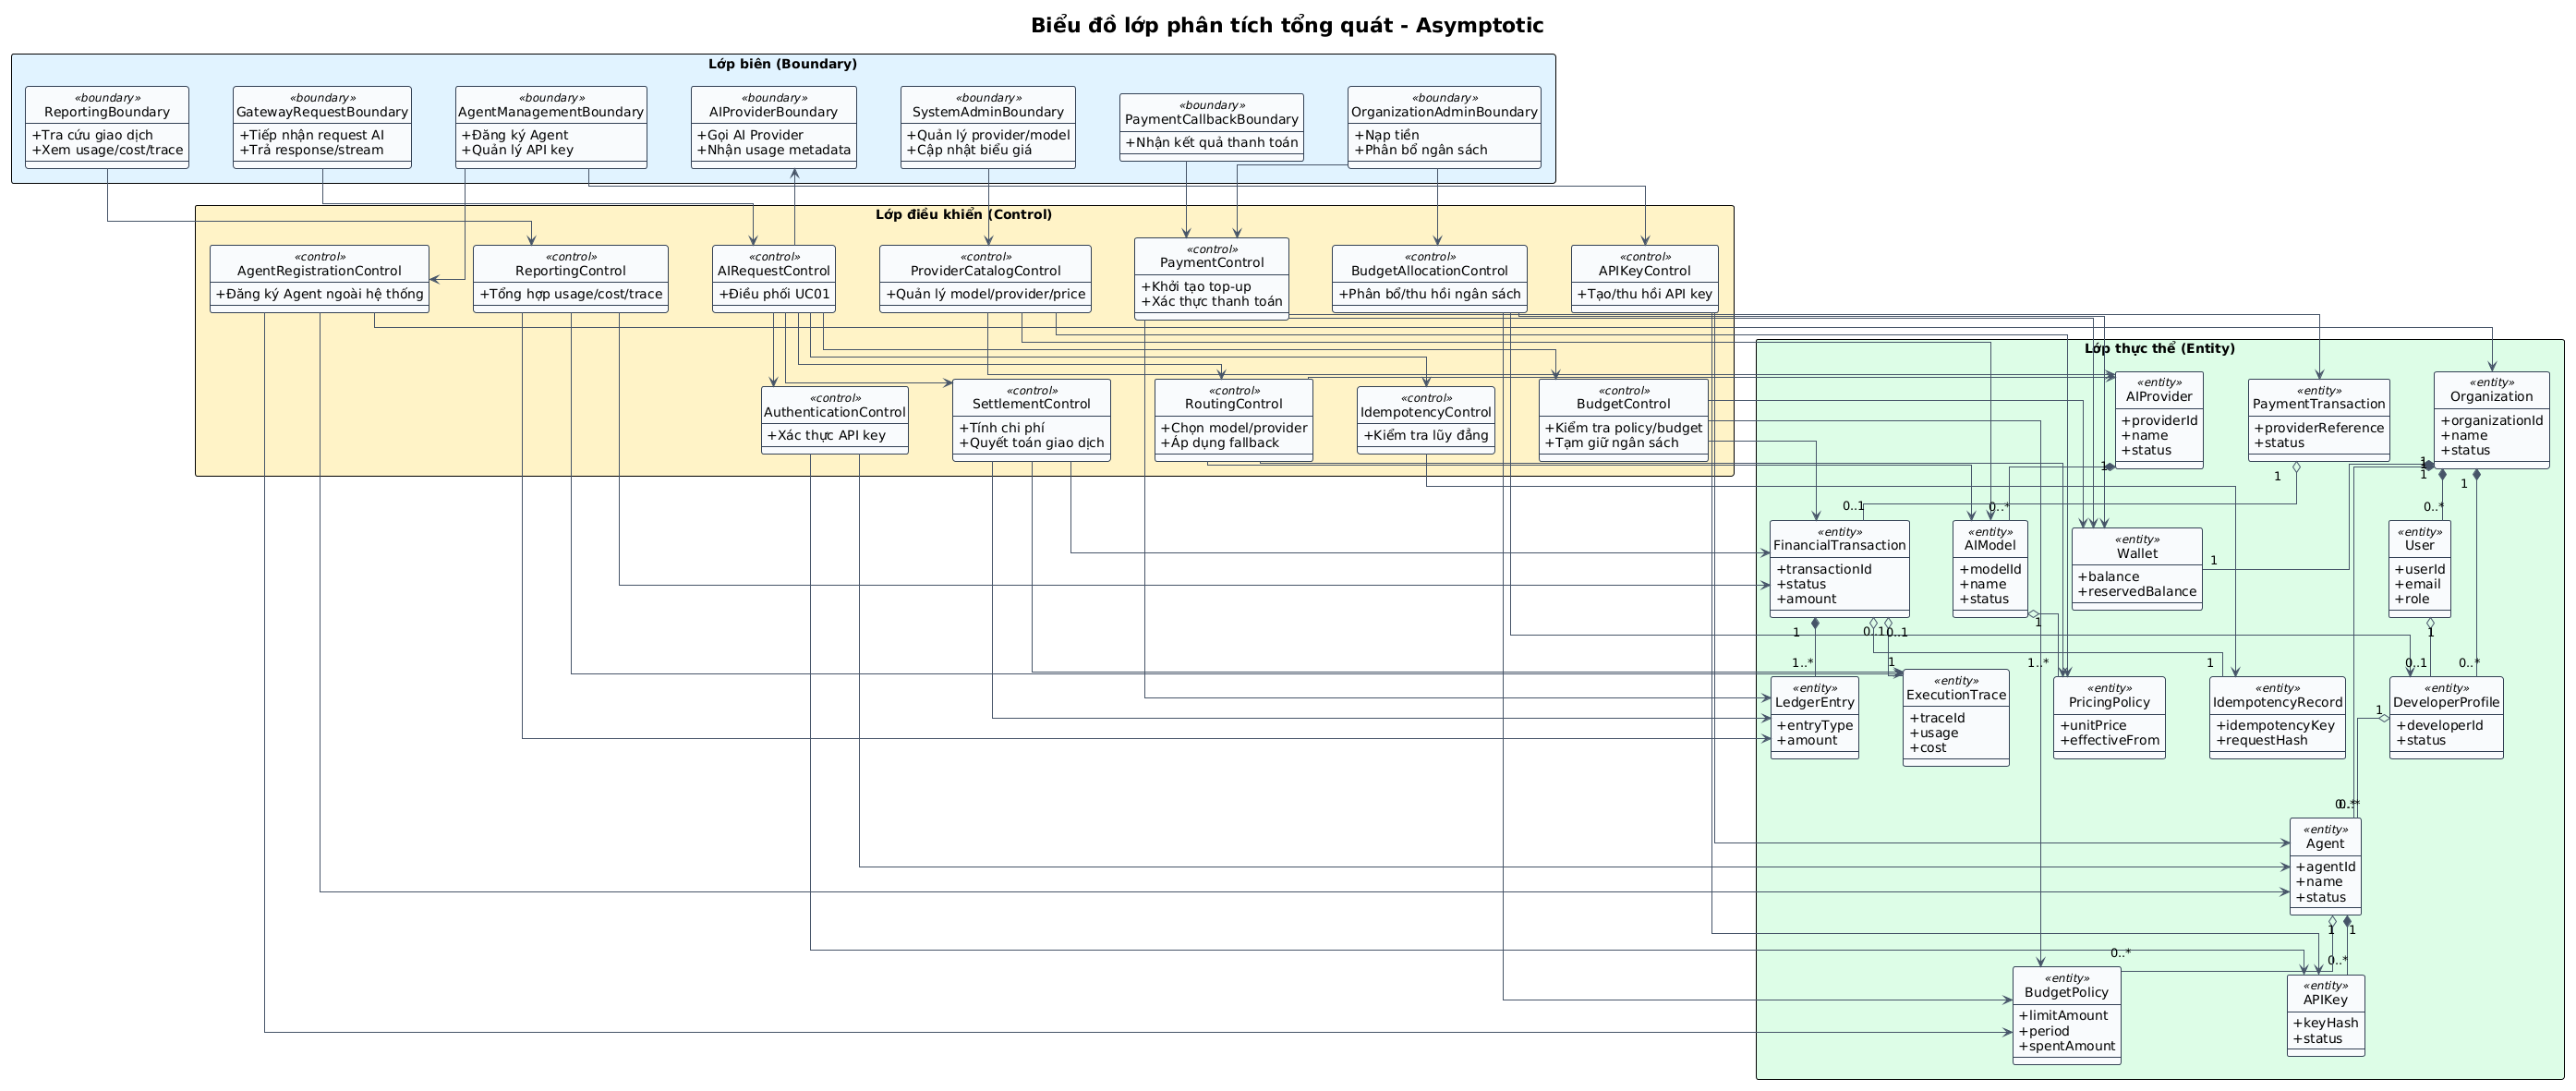
\includegraphics[width=0.98\textwidth,height=0.78\textheight,keepaspectratio]{report_support_documentation/class_diagram/diagram.png}
    \caption[Biểu đồ lớp phân tích tổng quát]{Biểu đồ lớp phân tích tổng quát của hệ thống. Nguồn: Tác giả xây dựng}\label{fig:analysis-class-diagram}
\end{figure}

\cref{fig:analysis-class-diagram} trình bày mô hình lớp phân tích tổng quát. Biểu đồ giữ ba nhóm lớp ở mức phân tích: lớp biên mô tả điểm tương tác, lớp điều khiển mô tả trách nhiệm điều phối use case và lớp thực thể mô tả trạng thái nghiệp vụ. Các quan hệ trên biểu đồ phản ánh sự phụ thuộc nghiệp vụ chính, không phải cấu trúc thư mục hay quan hệ gọi hàm ở mức mã nguồn.

\section{Phân tích lớp biên}

Lớp biên trong hệ thống đại diện cho ranh giới giữa Asymptotic và các actor hoặc hệ thống ngoài. Mỗi lớp biên được xác định theo kiểu tương tác, không theo công nghệ giao tiếp cụ thể.

\begin{longtable}{|L{0.28\textwidth}|L{0.30\textwidth}|L{0.32\textwidth}|}
\caption{Các lớp biên trong mô hình phân tích}\\
\hline
\textbf{Lớp biên} & \textbf{Actor/hệ thống liên quan} & \textbf{Trách nhiệm phân tích} \\
\hline
\endfirsthead
\hline
\textbf{Lớp biên} & \textbf{Actor/hệ thống liên quan} & \textbf{Trách nhiệm phân tích} \\
\hline
\endhead
\makecell[l]{GatewayRequest\\Boundary} & AI Agent & Tiếp nhận request AI từ Agent, trả kết quả hoặc lỗi, giữ vai trò điểm vào bắt buộc trước khi request được chuyển tới provider.\\
\hline
\makecell[l]{OrganizationAdmin\\Boundary} & Quản trị viên tổ chức, Lập trình viên & Tiếp nhận thao tác quản lý tổ chức, Agent, API key, ví, ngân sách và báo cáo trong phạm vi tổ chức.\\
\hline
\makecell[l]{SystemAdmin\\Boundary} & Quản trị viên hệ thống & Tiếp nhận thao tác cấu hình provider, model, endpoint, credential nội bộ, biểu giá và chính sách hệ thống.\\
\hline
\makecell[l]{PaymentCallback\\Boundary} & Payment Provider & Nhận kết quả thanh toán hoặc callback top-up để hệ thống xác thực và cập nhật trạng thái tài chính.\\
\hline
AIProviderBoundary & AI Provider & Đại diện ranh giới tích hợp với nhà cung cấp AI; Gateway sử dụng credential nội bộ khi gọi provider.\\
\hline
ReportingBoundary & Quản trị viên tổ chức, Lập trình viên & Cung cấp điểm truy cập dữ liệu usage, cost, transaction và trace theo quyền được cấp.\\
\hline
\end{longtable}

Điểm quan trọng là AI Agent chỉ tương tác với GatewayRequestBoundary bằng API key do Asymptotic cấp. Provider credential không đi qua lớp biên dành cho Agent và không được xem là dữ liệu mà Agent có thể quản lý.

\section{Phân tích lớp điều khiển}

Lớp điều khiển điều phối các bước nghiệp vụ của use case. Trong đề tài này, nhóm lớp điều khiển quan trọng nhất nằm ở luồng UC01, vì luồng này kết hợp xác thực, kiểm soát lũy đẳng, kiểm tra chính sách, kiểm tra ngân sách, định tuyến provider và quyết toán chi phí.

\begin{longtable}{|L{0.28\textwidth}|L{0.62\textwidth}|}
\caption{Các lớp điều khiển trong mô hình phân tích}\\
\hline
\textbf{Lớp điều khiển} & \textbf{Trách nhiệm phân tích} \\
\hline
\endfirsthead
\hline
\textbf{Lớp điều khiển} & \textbf{Trách nhiệm phân tích} \\
\hline
\endhead
AIRequestControl & Điều phối UC01 từ lúc nhận request tới lúc trả kết quả, đảm bảo các bước xác thực, lũy đẳng, ngân sách, định tuyến và ghi nhận trace diễn ra đúng thứ tự.\\
\hline
AuthenticationControl & Xác thực API key, xác định Agent, tổ chức chịu chi phí và phạm vi quyền tương ứng.\\
\hline
IdempotencyControl & Kiểm tra khóa lũy đẳng, phát hiện request gửi lại và ngăn ghi nhận chi phí trùng.\\
\hline
BudgetControl & Kiểm tra ngân sách, quota, policy và tạm giữ hoặc xác nhận hạn mức trước khi route request.\\
\hline
RoutingControl & Chọn provider/model phù hợp với request, chính sách và ngân sách; áp dụng fallback khi được cấu hình.\\
\hline
SettlementControl & Ghi nhận usage/cost sau khi provider trả kết quả, quyết toán giao dịch, giải phóng phần tạm giữ dư và cập nhật trace.\\
\hline
AgentAccessControl & Điều phối đăng ký AI Agent bên ngoài, cập nhật trạng thái Agent, quản lý API key và gắn Agent với chính sách sử dụng.\\
\hline
PaymentControl & Điều phối top-up, xác thực kết quả thanh toán, cập nhật ví tổ chức và ghi nhận bút toán tương ứng.\\
\hline
\makecell[l]{BudgetAllocation\\Control} & Phân bổ hoặc thu hồi ngân sách giữa ví tổ chức, lập trình viên, nhóm hoặc Agent theo quyền quản trị.\\
\hline
ReportingControl & Tổng hợp usage, cost, transaction và trace theo phạm vi quyền truy cập.\\
\hline
\makecell[l]{ProviderCatalog\\Control} & Điều phối quản lý provider, model, endpoint, biểu giá và credential nội bộ của Gateway.\\
\hline
\end{longtable}

Các lớp điều khiển không thay thế lớp thực thể. Chúng sử dụng lớp thực thể để đọc hoặc cập nhật trạng thái nghiệp vụ, đồng thời bảo đảm mỗi use case có một điểm điều phối rõ ràng.

\section{Phân tích lớp thực thể}

Lớp thực thể biểu diễn trạng thái nghiệp vụ cần được bảo toàn qua nhiều use case. Trong hệ thống này, các thực thể tài chính và truy vết giữ vai trò đặc biệt quan trọng vì request do AI Agent có thể phát sinh tự động, song song và khó dự đoán trước chi phí.

\begin{longtable}{|L{0.28\textwidth}|L{0.62\textwidth}|}
\caption{Các lớp thực thể trong mô hình phân tích}\\
\hline
\textbf{Lớp thực thể} & \textbf{Ý nghĩa nghiệp vụ} \\
\hline
\endfirsthead
\hline
\textbf{Lớp thực thể} & \textbf{Ý nghĩa nghiệp vụ} \\
\hline
\endhead
Organization & Tổ chức sử dụng Gateway, là phạm vi sở hữu ví, người dùng, lập trình viên, Agent và chi phí.\\
\hline
User & Cá nhân có danh tính trong hệ thống, được gán vai trò trong tổ chức hoặc vai trò quản trị hệ thống.\\
\hline
DeveloperProfile & Hồ sơ lập trình viên thuộc tổ chức, có thể đăng ký Agent và nhận phạm vi ngân sách được cấp.\\
\hline
Agent & AI Agent bên ngoài được đăng ký vào Gateway; Agent không được tạo, huấn luyện hoặc vận hành bởi hệ thống.\\
\hline
APIKey & Khóa truy cập do Asymptotic cấp cho Agent để gọi Gateway; khóa được quản lý tách biệt với provider credential.\\
\hline
Wallet & Ví hoặc ngân sách khả dụng của tổ chức, phản ánh số dư, phần đã tạm giữ và khả năng chi trả.\\
\hline
BudgetPolicy & Chính sách hạn mức, quota hoặc budget áp dụng cho tổ chức, lập trình viên, Agent hoặc phạm vi sử dụng.\\
\hline
AIProvider & Nhà cung cấp dịch vụ AI trả phí mà Gateway có thể gọi bằng credential nội bộ.\\
\hline
AIModel & Mô hình hoặc endpoint cụ thể thuộc một AI Provider, có trạng thái hỗ trợ và chính sách giá tương ứng.\\
\hline
PricingPolicy & Quy tắc đơn giá hoặc chi phí dự kiến dùng để ước lượng và quyết toán chi phí request.\\
\hline
FinancialTransaction & Giao dịch tài chính đại diện cho top-up, phân bổ, tạm giữ, quyết toán, hoàn trả hoặc lỗi cần đối soát.\\
\hline
LedgerEntry & Bút toán ghi nhận biến động tài chính ở dạng có thể truy vết và đối soát.\\
\hline
PaymentTransaction & Giao dịch với Payment Provider, dùng để xác thực và ghi nhận kết quả nạp tiền.\\
\hline
IdempotencyRecord & Bản ghi lũy đẳng liên kết khóa gửi lại, nội dung request và kết quả đã xử lý.\\
\hline
ExecutionTrace & Nhật ký thực thi request AI, lưu trạng thái, provider/model, usage, cost và thông tin phục vụ báo cáo.\\
\hline
\end{longtable}

Nhóm thực thể trên cho thấy trọng tâm của hệ thống không nằm ở việc tự tạo AI Agent, mà ở việc kiểm soát tài chính, truy cập và trace cho Agent bên ngoài khi Agent sử dụng dịch vụ AI trả phí qua Gateway.

\section{Đối chiếu lớp phân tích với trường hợp sử dụng}

Bảng đối chiếu trong mục này chứng minh mỗi use case chính đều có lớp biên, lớp điều khiển và thực thể nghiệp vụ tương ứng. Đây là cầu nối từ Chương 2 sang thiết kế lớp và thiết kế tương tác ở Chương 4.

{\footnotesize
\begin{longtable}{|L{0.08\textwidth}|L{0.32\textwidth}|L{0.28\textwidth}|L{0.22\textwidth}|}
\caption{Đối chiếu trường hợp sử dụng với lớp phân tích}\\
\hline
\textbf{Use Case} & \textbf{Lớp biên} & \textbf{Lớp điều khiển} & \textbf{Lớp thực thể chính} \\
\hline
\endfirsthead
\hline
\textbf{Use Case} & \textbf{Lớp biên} & \textbf{Lớp điều khiển} & \textbf{Lớp thực thể chính} \\
\hline
\endhead
UC01 & GatewayRequestBoundary,\newline AIProviderBoundary & AIRequestControl,\newline AuthenticationControl,\newline IdempotencyControl,\newline BudgetControl, RoutingControl,\newline SettlementControl & Agent, APIKey, Wallet,\newline BudgetPolicy, AIProvider,\newline AIModel, FinancialTransaction,\newline LedgerEntry, IdempotencyRecord,\newline ExecutionTrace\\
\hline
UC02 & OrganizationAdminBoundary,\newline PaymentCallbackBoundary & PaymentControl & Organization, Wallet,\newline PaymentTransaction,\newline FinancialTransaction, LedgerEntry\\
\hline
UC03 & OrganizationAdminBoundary & BudgetAllocationControl,\newline BudgetControl & Organization, DeveloperProfile,\newline Agent, Wallet, BudgetPolicy,\newline FinancialTransaction, LedgerEntry\\
\hline
UC04 & OrganizationAdminBoundary & AgentAccessControl,\newline BudgetAllocationControl & Organization, DeveloperProfile,\newline Agent, BudgetPolicy\\
\hline
UC05 & OrganizationAdminBoundary & AgentAccessControl,\newline AuthenticationControl & Agent, APIKey,\newline DeveloperProfile, Organization\\
\hline
UC06 & ReportingBoundary & ReportingControl & FinancialTransaction,\newline LedgerEntry, ExecutionTrace,\newline Agent, Organization\\
\hline
UC07 & OrganizationAdminBoundary & AgentAccessControl & User, Organization, Wallet\\
\hline
UC08 & OrganizationAdminBoundary & AgentAccessControl,\newline BudgetAllocationControl & User, DeveloperProfile,\newline Organization, BudgetPolicy,\newline Agent, APIKey\\
\hline
UC09 & SystemAdminBoundary & ProviderCatalogControl,\newline RoutingControl & AIProvider, AIModel, PricingPolicy\\
\hline
\end{longtable}
}

Qua bảng đối chiếu, các use case tài chính đều liên kết tới ví, giao dịch tài chính và bút toán; các use case liên quan Agent đều liên kết tới Agent và APIKey; các use case định tuyến provider đều liên kết tới AIProvider, AIModel và PricingPolicy. Sự nhất quán này là cơ sở để thiết kế package, service, repository, adapter và sequence diagram ở chương tiếp theo.

\section*{Kết luận chương}

Chương này đã xác định mô hình lớp phân tích của Asymptotic theo Boundary--Control--Entity. Các lớp biên thể hiện ranh giới tương tác với actor và hệ thống ngoài, các lớp điều khiển thể hiện trách nhiệm điều phối use case, còn các lớp thực thể thể hiện trạng thái nghiệp vụ cần bảo toàn. Kết quả phân tích này làm nền cho Chương 4, nơi các lớp phân tích được chuyển thành thiết kế gói, lớp thiết kế, tương tác, trạng thái, dữ liệu và API.
